\pdfoutput=1
\documentclass{article}

\input{preamble/preamble.tex}
\input{preamble/preamble_math}
\input{preamble/definitions_basic}

\input{preamble/minimalist_biblatex}

\addbibresource{bibs/refs.bib}

\crefformat{equation}{(#2#1#3)}
\crefformat{figure}{Figure~#2#1#3}
\crefname{example}{Example}{Examples}
\crefname{lemma}{Lemma}{Lemmas}
\crefname{cor}{Corollary}{Corollaries}
\crefname{theorem}{Theorem}{Theorems}
\crefname{assumption}{Assumption}{Assumptions}

\usepackage{enumitem}
\usepackage[separate-uncertainty=true,multi-part-units=single]{siunitx}

\usepackage{xcolor}
\input{preamble/commenting.tex}

\usepackage[affil-it]{authblk}

\title{Affective Factors Predict Selective Attention\\in Vision-Language Models}
\date{}
\author[1]{Michael Zhu}
\affil[1]{Master in Computational Social Science}

\begin{document}
\maketitle

\begin{abstract}
Vision-language models are often expected to form comprehensive and objective
representations of visual scenes, 
yet recent work suggests that models such as CLIP encode some content more strongly than others. 
Here, we ask whether such selective attention is shaped by the affective properties of visual content.
In human attention, emotionally arousing stimuli tend to capture attention more readily than neutral stimuli.
We tested whether a similar arousal bias appears in CLIP visual encoders. 
We presented six ViT-based CLIP models with composite stimuli containing pairs of affective images and quantified attentional priority using two complementary metrics. 
Image-level regressions showed that arousal consistently predicted model attentional priority across all models, metrics, and datasets, even after controlling for low-level visual features. 
Valence effects were weaker and less consistent.
These results suggest that large-scale multimodal training may transmit not
only visual-semantic knowledge, but also human-like affective biases in what
visual content receives priority.
\end{abstract}

%----------------------------------------------------------------------
\section{Introduction}
%----------------------------------------------------------------------
Many practical applications of vision-language models expect comprehensive, objective representations of visual scenes. However, research has shown that vision-language models such as CLIP do not encode visual content equally, but instead exhibit systematic differences in attentional priority. For example, \citet{abbasiCLIPMicroscopeFineGrained2025} found that in multi-object retrieval tasks, CLIP's image encoder is biased toward larger objects, while its text encoder is biased toward objects mentioned earlier. These findings suggest that CLIP's representations are not evenly balanced, but are instead shaped by presentational factors such as object size and order of mention. Yet presentational factors alone cannot fully address a deeper question: does CLIP also have intrinsic preferences driven by content itself? %That is, when different content is presented in the same way and controlled for low-level visual features, does the model still prioritize certain types of content?

The visual world contains far more information than can be processed at once, so humans rely on selective attention to prioritize some content while suppressing the rest \citep{tresilianSelectiveAttentionReaching1999,serencesSelectiveVisualAttention2006,desimoneNeuralMechanismsSelective1995}. A large body of human research has shown that emotionally salient content tends to win out in attentional competition. High-arousal stimuli---whether threatening or exciting---are generally more likely to capture attention than neutral stimuli, a phenomenon often described as arousal-biased competition \citep{hansenFindingFaceCrowd1988a,ohmanEmotionDrivesAttention2001,vogtAllocationSpatialAttention2008b,schimmackAttentionalInterferenceEffects2005a}.

We propose that a similar affective attentional bias may be inherited by vision-language models through their training process. Models such as CLIP are trained on large-scale human-generated image--text pairs \citep{radfordLearningTransferableVisual2021a}. Image captions are usually not exhaustive records of visual scenes, but selective ones: people tend to describe what they find most salient and noteworthy. If high-arousal content is more likely to capture human attention and thus more likely to be mentioned in captions, contrastive image--text training may push models to assign such content higher attentional priority. 

In the present study, we test this possibility by examining whether human affective ratings predict CLIP’s attentional priority across competing visual content.
%In this way, models may learn not only the semantic correspondences between images and text, but also the attentional biases embedded in human description behavior.

%This hypothesis also connects to a broader question about the relation between model representations and human affect. Prior work has shown that visual model representations can predict human affective responses to images \citep{conwellPerceptualPrimacyFeeling2025}. However, this line of research is primarily about whether models encode affectively relevant information. Our question is different: when multiple images compete for representation, do the affective properties of those images influence which one the model prioritizes? We are therefore not asking whether models can represent emotional content, but whether emotion shapes a downstream consequence---that is, which content gets encoded more.

%To examine this, we constructed composite stimuli by placing pairs of affectively rated images side by side and presented them to six CLIP models with ViT-based visual encoders. We quantified how models allocated attentional priority using two complementary metrics: within-constituent attention rollout and composite-constituent embedding similarity. Image-level regression analyses showed that arousal consistently predicted model attentional priority across models, metrics, and datasets, while the effect of valence was weaker and less consistent. These findings suggest that vision-language models may not only learn visual-semantic knowledge, but also inherit human-like affective attentional biases.

%----------------------------------------------------------------------
\section{Methods}
%----------------------------------------------------------------------

\subsection{Models}

We evaluated six CLIP models with ViT-based visual encoders from the OpenCLIP
library~\citep{cherti2023reproducible, ilharco_gabriel_openclip_repo}.
The models vary along two dimensions: architectural scale (ViT-B/32, ViT-B/16, ViT-L/14) and pretraining dataset 
(LAION-2B and DataComp-1B), 
giving a $3 \times 2$ design. 
We analyzed only the CLIP visual encoder and excluded the text pathway, since our question concerns visual attentional priority.


\subsection{Datasets}
\parhead{OASIS (primary).}
The Open Affective Standardized Image Set
(OASIS;~\citep{kurdiIntroducingOpenAffective2017}) contains 900 color images
spanning people, animals, objects, and landscapes. Each image has normative
valence and arousal ratings collected online from approximately 100 MTurk
participants, with high inter-rater reliability
($r_\text{valence} = .984$, $r_\text{arousal} = .929$). For examples, see \cref{fig:affective_space_examples}. 

\parhead{Supplementary datasets.}
EmoMadrid~\citep{carretieEmoMadridEmotionalPictures2019} contains 813
color photographs spanning animals, objects, food, landscapes, and people.
Each image has normative valence and arousal ratings collected in-person from over 700
participants across multiple evaluation sessions, with all test-retest
reliabilities above $0.9$.
The Nencki Affective Picture System
(NAPS;~\citealt{marchewkaNAPSIntroduction2014}) contains 1,356 color
photographs spanning people, faces, animals, objects, and landscapes. Each image has
normative valence and arousal ratings collected from 204 participants.

We chose OASIS as our primary dataset for three reasons. 
First, its images span a broad affective space with near-zero correlation between valence and arousal ($r = -.06$; \cref{fig:distribution}), minimizing the collinearity in the
regression analysis. 
In contrast, valence and arousal are substantially
correlated in the supplementary datasets (NAPS: $r = -.82$; EmoMadrid:
$r = -.58$). 
Second, all OASIS images share the same near-square size
($500 \times 400$ pixels), making them well-suited to patch-aligned composite construction without large distortion. 
In contrast, images in the other two datasets have varying non-square ratios. 
Third, OASIS places no restrictions on image display and provides a concept label for each image, allowing us to present both image-level instances and concept-level summaries.

\subsection{Stimuli Construction}

In each trial, the model received a composite image containing two constituent images placed side by side on a white square canvas. 
Each constituent was resized to occupy exactly $5 \times 5$ ViT patches, with one patch of white padding between them. 
The full canvas is therefore $11 \times 11$ patches, with both images vertically centered (\cref{fig:schematic}).
This ensures that each constituent occupies an integer number of patches with no boundary ambiguity, so that attention rollout values can be cleanly attributed to each constituent region.

For each dataset, we randomly sampled 100,000 ordered image pairs, allowing each image to appear across diverse pairing contexts and positions.

\begin{figure}[t]
  \centering
  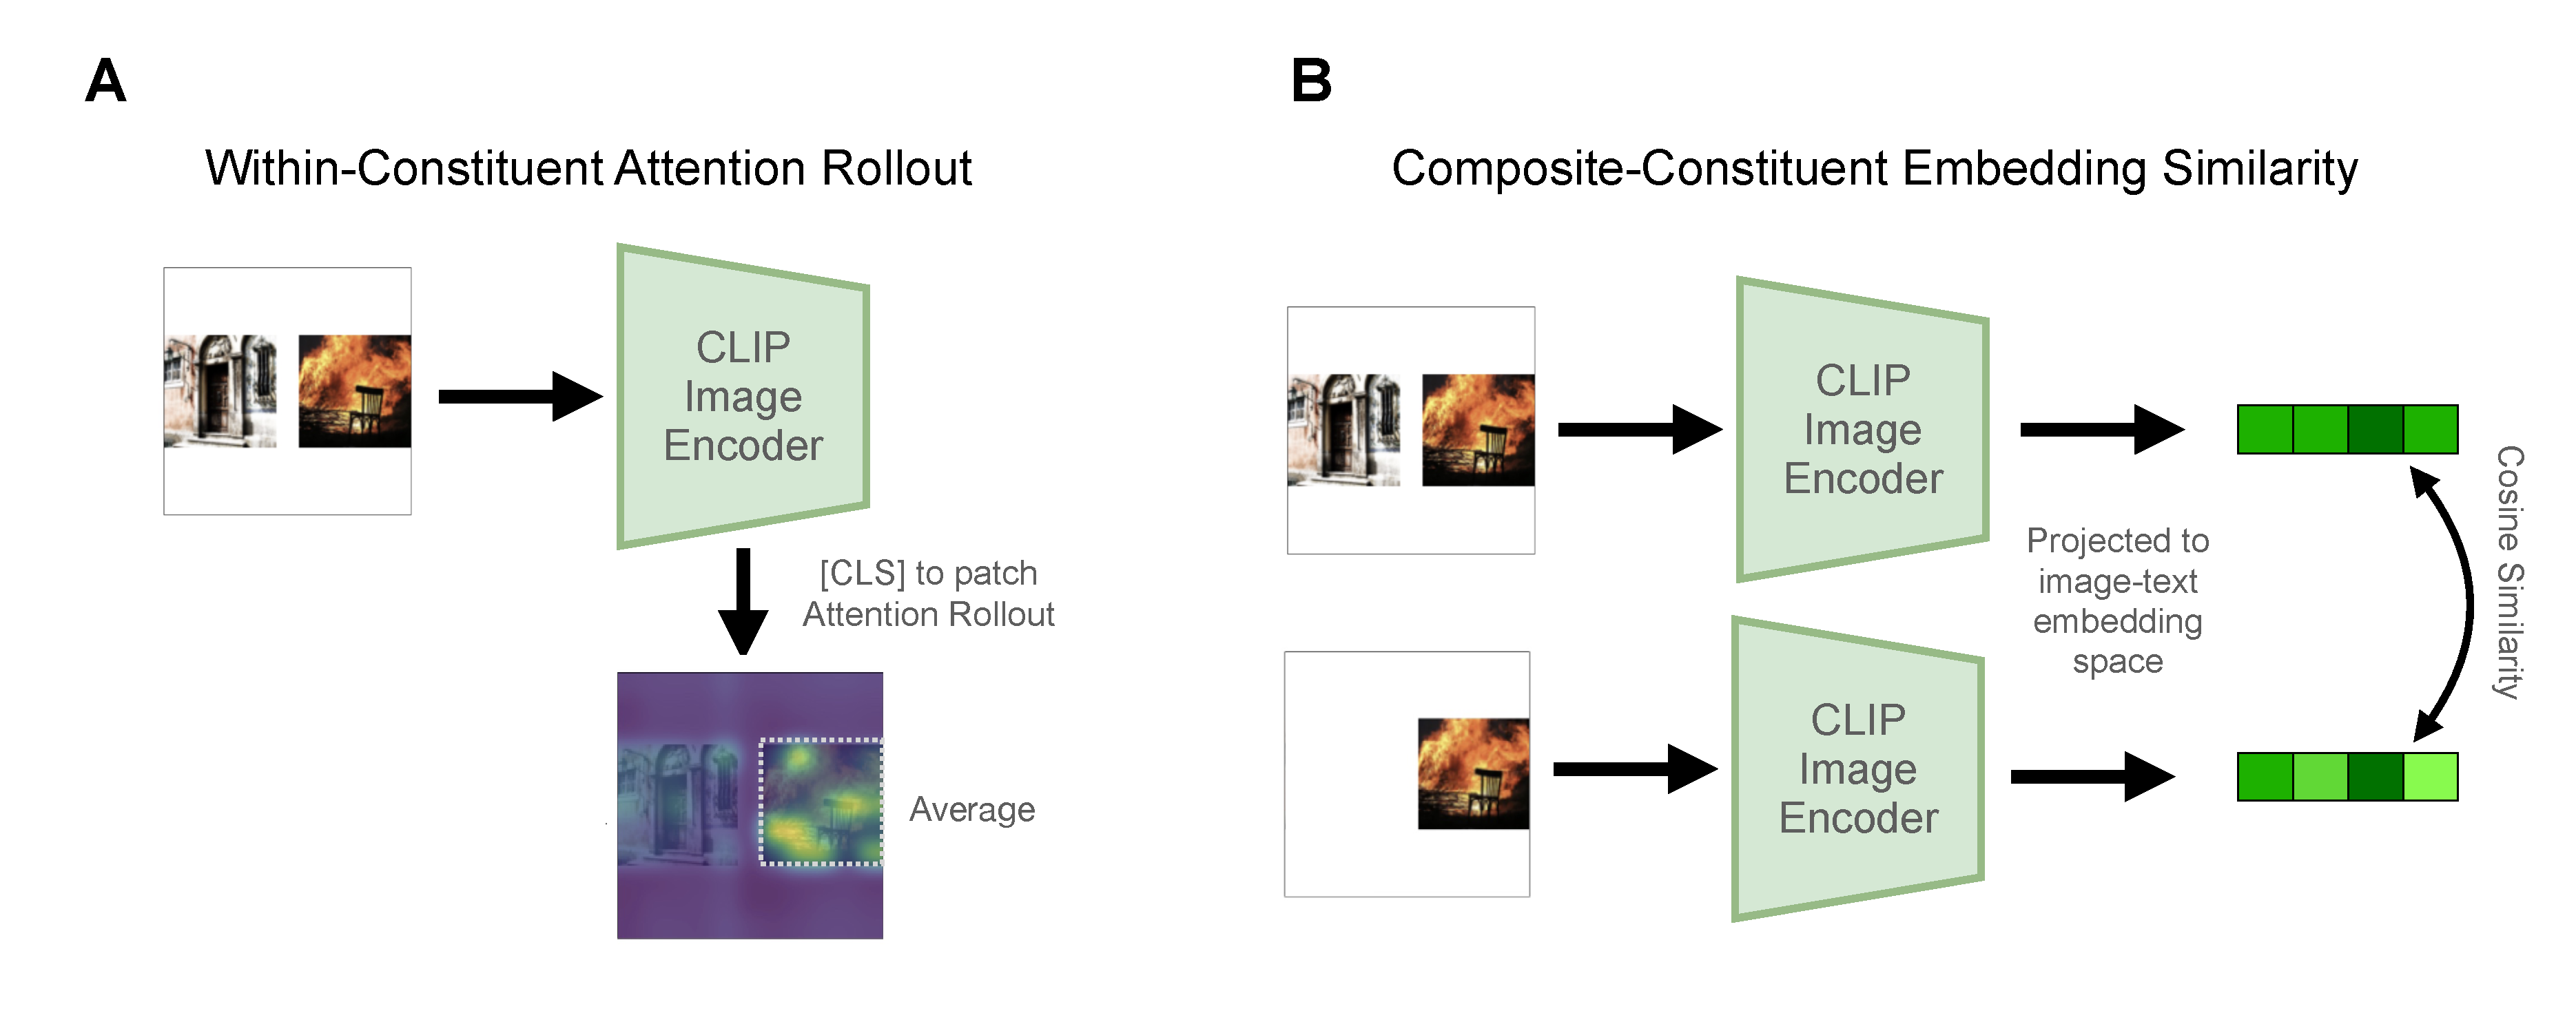
\includegraphics[width=\textwidth]{plots/Fig1_schematic.pdf}
  \caption{Two complementary metrics of attentional priority in CLIP visual
    encoders. 
    \textbf{(A)} Within-constituent attention rollout: a rollout map is computed from the \texttt{[CLS]} token to all image patches, and values are averaged within each constituent's patch region. 
    \textbf{(B)}
    Composite-constituent embedding similarity: the cosine similarity between
    the composite's embedding and each constituent's embedding.}
  \label{fig:schematic}
\end{figure}

\subsection{Attentional Priority Metrics}

We used two complementary metrics to quantify model attentional priority
(\cref{fig:schematic}).

\parhead{Within-constituent attention rollout.}
Attention rollout~\citep{attentionrollout_abnar2020} estimates cumulative
information flow among tokens. It recursively multiplies attention matrices across transformer layers, incorporating residual connections. For layer $l$ with attention matrix $A^{(l)}$
\begin{align}
  \tilde{A}^{(l)} &= \mathrm{normalize}\!\left(A^{(l)} + I\right), \\
  R &= \tilde{A}^{(L)} \tilde{A}^{(L-1)} \cdots \tilde{A}^{(1)}.
\end{align}
$R_{q,p}$ summarizes the cumulative attention flow from query token $q$
to key token $p$ across all layers. Before computing rollout, multi-head
attention weights are aggregated by taking the maximum across heads, and a
discard ratio of 0.7 removes low-attention connections except those involving \texttt{[CLS]}.

To obtain a constituent-level measure, we used the \texttt{[CLS]} row of the rollout matrix and averaged its values over all patch tokens belonging to constituent $i$. 
Let $M_i$ denote the set of patch tokens in constituent
$i$'s spatial region. The rollout of constituent $i$ is
\begin{equation}
  s_i = \frac{1}{\abs{M_i}} \sum_{p \in M_i} R_{\texttt{CLS},\, p}.
\end{equation}
Higher rollout indicates greater cumulative influence of the constituent on the final \texttt{[CLS]} representation, as estimated from the layer-wise attention flow in the visual encoder.

\parhead{Composite--constituent embedding similarity.}
We also measured how similar the composite image's embedding is to each
constituent's embedding. Here, the embedding refers to the image feature
projected into CLIP's joint image--text embedding space, as returned by
\texttt{encode\_image()}.

For each trial, we extracted the embeddings of the composite image and each constituent image. 
To control for background and position, each constituent was presented alone in its original spatial position, as in the composite (\cref{fig:schematic}B). 
We then computed the cosine similarity between the composite embedding and each constituent embedding.

Higher similarity indicates that the composite representation more closely
resembles that constituent representation in CLIP's joint embedding space.

\subsection{Image-level Priority and Regression}

Within each trial, constituent scores of each metric were normalized to sum to 1, giving
relative priorities $\tilde{s}_i = s_i / (s_i + s_j)$. Each image's overall
attentional priority was defined as the mean $\tilde{s}_i$ across all trials in which it appeared.

We fit an image-level regression for each combination of dataset, model, and metric:
\begin{equation}
\label{eq:regression}
  \mathrm{Priority} \;\sim\;
  \mathrm{Arousal} + \mathrm{Valence} +
  \mathrm{Contrast} + \mathrm{Entropy} +
  \mathrm{Ldim} + \mathrm{Adim} + \mathrm{Bdim}.
\end{equation}
This model tested whether affective factors, namely arousal and valence,
predicted attentional priority. We controlled for low-level visual features:
contrast (standard deviation of grayscale pixel intensity), entropy
(complexity of the grayscale intensity distribution), and three CIELAB color
channels (Ldim: lightness; Adim: red--green; Bdim: yellow--blue).

All reported coefficients are standardized coefficients. All $p$-values were Bonferroni-corrected
across the full set of planned tests.

%----------------------------------------------------------------------
\section{Results}
%----------------------------------------------------------------------

\subsection{What Receives High Attentional Priority?}

Before examining regression coefficients, we first inspected which items received high or low attentional priority.
Because OASIS is the only dataset that permits image display and provides concept labels, we restricted this visualization to OASIS.

For each model--metric combination, we converted image-level priority scores to ranks. We then averaged these ranks across models and metrics, yielding one mean priority rank for each image. 

\begin{figure}[h]
  \centering
  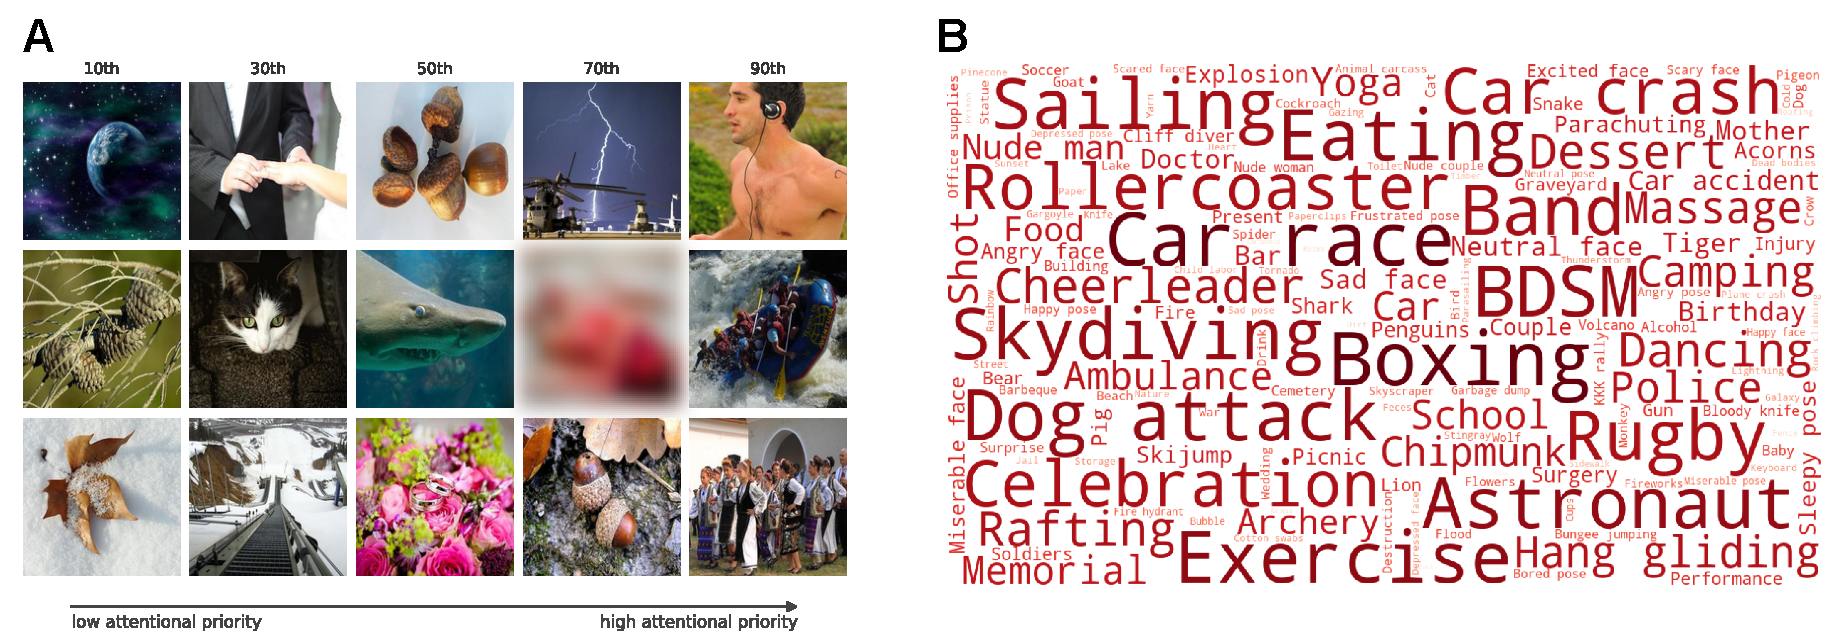
\includegraphics[width=\textwidth]{plots/Fig2_instances.pdf}
  \caption{OASIS images and concept labels associated with attentional priority.
  \textbf{(A)} Representative images from the 10th to 90th priority percentiles (left to right), based on rank-normalized scores averaged across all model $\times$ metric combinations. One disturbing image depicting a bloody carcass was blurred.
  \textbf{(B)} Concept-level word cloud generated by averaging priority ranks across images under the same concept label. Larger font size and darker color indicate higher mean priority rank.}
  \label{fig:instances}
\end{figure}

\Cref{fig:instances}A shows representative images at different priority
percentiles. 
Low-priority images tend to depict static or low-arousal content, such as pine cones, a road leading to the distance, or a leaf in snow. 
In contrast, high-priority images more often depict action, threat, or emotionally intense content, such as lightning with helicopters, a bloody carcass (blurred), and rafting in flood water.

To summarize priority at the concept level, we further averaged image ranks within each OASIS concept label, restricting to concepts with more than one image instance.
\cref{fig:instances}B shows the resulting word cloud, where font size and color intensity both reflect mean concept-level priority rank. 
High-arousal concepts stand out, such as \emph{Rollercoaster},
\emph{Skydiving}, \emph{Celebration}, \emph{Car race}, \emph{Dog attack}, and \emph{Boxing}.



\subsection{Affective Factors Predict Attentional Priority}

We next tested whether affective ratings predicted image-level attentional priority after controlling for low-level visual features. \Cref{fig:oasis_coefs} shows standardized regression coefficients for OASIS across six CLIP models and two attentional priority metrics.

Arousal shows a consistent positive effect. 
Across all models and both metrics, higher arousal predicts higher attentional priority, even after controlling for visual features.
Standardized coefficients are approximately $.20$--$.30$.

Valence shows a weaker and metric-dependent pattern. 
For attention rollout, valence has standardized coefficients of roughly $.15$ across models, indicating that more positive images tend to receive higher rollout priority after visual controls. 
For embedding similarity, however, valence coefficients are close to zero and are not significant.

\begin{figure}[h]
  \centering
  
\includegraphics[width=\textwidth]{plots/Fig3_coef_OASIS.pdf}
  \caption{Standardized coefficients predicting image-level attentional priority for OASIS. 
  Each point shows the coefficient from one CLIP model. 
  Row panels correspond to the two attentional priority metrics. 
  All $p$-values are Bonferroni-corrected across all planned tests. Filled dots indicate corrected $p < .05$; open circles indicate non-significant effects.}
  \label{fig:oasis_coefs}
\end{figure}

Visual features show stronger effects for attention rollout than for embedding similarity, although most effects have similar directions across metrics.\fTBD{The main exception is Ldim, which shows a positive effect for embedding similarity. This may be due to our white-background setup: brighter images are more similar to the background and may therefore yield higher embedding similarity.} 
Overall, this pattern suggests that rollout is more sensitive to low-level visual properties. This is expected because rollout is computed within the visual encoder, whereas embedding similarity is measured in CLIP's joint image--text embedding space. 
Nevertheless, the positive arousal effect remains consistent across both metrics.

\subsection{Cross-Dataset Robustness}

To test whether the results generalize beyond OASIS, we repeated the experiments using NAPS and EmoMadrid as independent stimulus sets.

\Cref{fig:landscape} visualizes model attentional priority across the
valence--arousal space for all three datasets and both metrics. 
Across datasets and metrics, high-priority regions tend to concentrate at higher arousal values, consistent with the regression results from OASIS. Valence also shows a positive trend, but the pattern is less pronounced than arousal.

\begin{figure}[t]
  \centering
  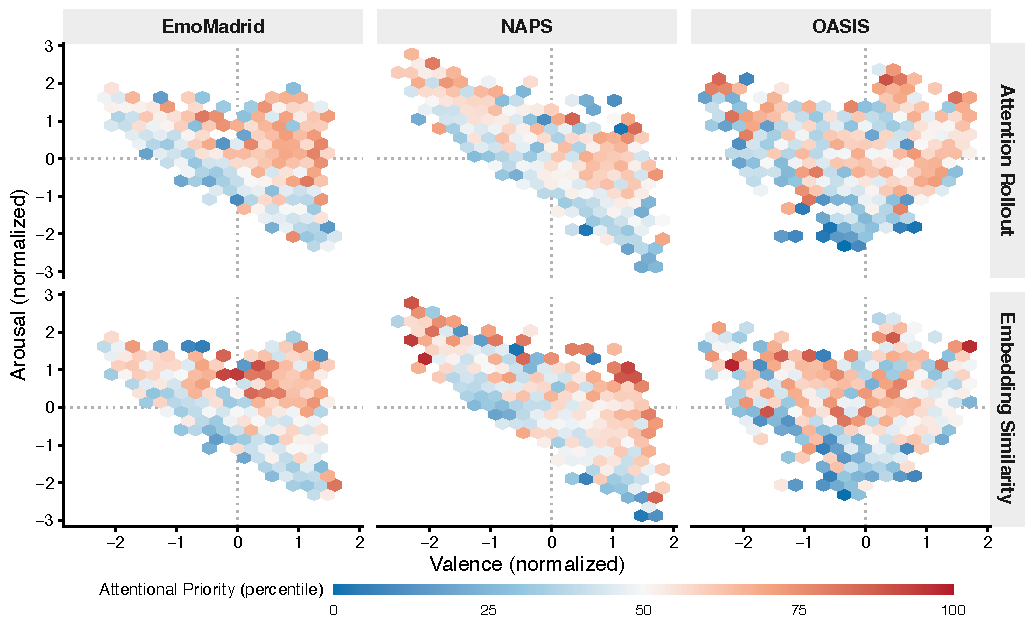
\includegraphics[width=\textwidth]{plots/Fig4_affect_landscape.pdf}
  \caption{Affective landscape of model attentional priority across datasets and metrics. 
  Each hex represents a local region of the normalized valence
  ($x$-axis) by arousal ($y$-axis) space. 
  Color encodes the mean attentional-priority percentile within that hex (blue = low, red = high).}
  \label{fig:landscape}
\end{figure}

\Cref{fig:cross_dataset} shows the affective standardized coefficients for the three datasets. 
In most model--metric combinations, both arousal and valence positively predict attentional priority, with the main exception being embedding similarity in OASIS.
Full coefficient plots including visual features for EmoMadrid and NAPS are provided in \cref{fig:coef_emomadrid} and \cref{fig:coef_naps}.

\begin{figure}[h]
  \centering
  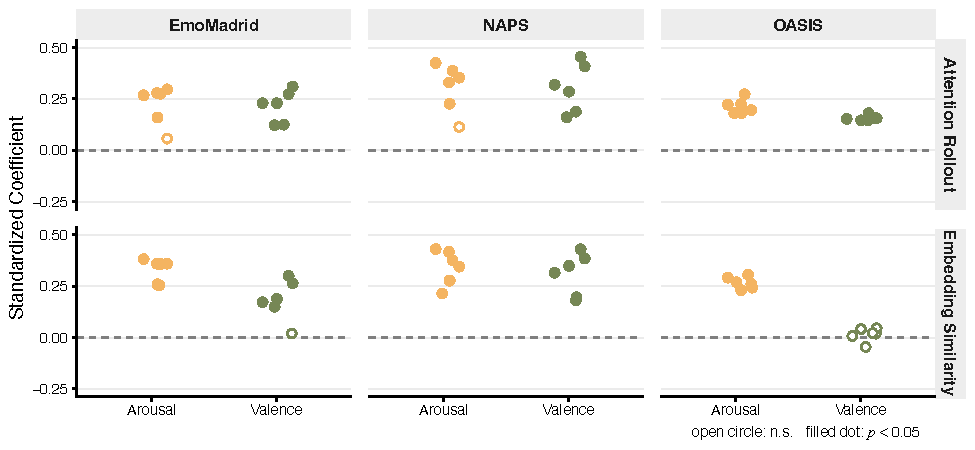
\includegraphics[width=\textwidth]{plots/Fig5_coef_cross_dataset.pdf}
  \caption{Affective standardized coefficients across datasets and metrics.
  Filled dots: Bonferroni-corrected $p < .05$; open circles: n.s.}
  \label{fig:cross_dataset}
\end{figure}

%----------------------------------------------------------------------
\section{Discussion}
%----------------------------------------------------------------------

In this study, we investigated whether vision-language models exhibit human-like affective biases in visual selective attention. We presented six ViT-based CLIP models with composite stimuli containing side-by-side affective images, and quantified attentional priority using two complementary metrics: within-constituent attention rollout and composite-constituent embedding similarity. Across six models, two priority metrics, and three image sets, we found that human arousal ratings consistently predicted model attentional priority, even after controlling for low-level visual features. Valence ratings also showed positive effects, but these effects were weaker and less consistent.

This arousal effect resembles the well-documented arousal competition in human attention \citep{vogtAllocationSpatialAttention2008b, schimmackAttentionalInterferenceEffects2005a, hansenFindingFaceCrowd1988a, ohmanEmotionDrivesAttention2001}, and this effect remained robust even when low-level visual properties were controlled. One plausible explanation is that this bias is inherited from human-generated training data. Image captions are selective rather than exhaustive: people tend to describe some parts of a scene while omitting others. If emotionally arousing content is more likely to be noticed and thus mentioned in captions, large-scale image--text contrastive training may encourage the model to assign greater priority to such content. Future work can test this hypothesis in two ways. First, comparing self-supervised vision models with vision-language models would help clarify whether description input is necessary for the effect. Second, analyzing training data could test whether emotionally salient content is more likely to be mentioned in captions compared to neutral content.

The positive valence effect is somewhat surprising, since human attention research often emphasizes attentional priority for negative or threatening stimuli \citep{prattoAutomaticVigilanceAttentiongrabbing1991, hansenFindingFaceCrowd1988a, ohmanEmotionDrivesAttention2001}, or reports no reliable effect of valence \citep{schimmackAttentionalInterferenceEffects2005a, vogtAllocationSpatialAttention2008b}. One possibility is that there is a gap between description and attention. Negative high-arousal content may capture attention but also elicit avoidance, leading people to describe it less. In contrast, positive emotion may broaden awareness \citep{fredrickson2004broaden}, leading people to attend to more content in an image and describe more of it.  Another possibility concerns data curation and censorship. Extremely violent, bloody, or disgusting images may be less likely to be posted online, or may be filtered out of curated training datasets, as in \citep{radfordLearningTransferableVisual2021a}, which could weaken the representation of negative high-arousal content in model training. This account may also help explain why nudity did not stand out among high-priority OASIS examples in \cref{fig:instances}.

This project also has several limitations. First, our side-by-side composite design provides strict experimental control, but it may not fully capture selective attention in natural multi-object scenes. Future work could examine whether similar affective effects appear in more naturalistic scenes, such as analyzing attention allocation when processing movie frames. Second, the affective datasets themselves impose constraints on interpretation. Except for OASIS, the datasets used here show substantial correlations between valence and arousal, which makes the independent contribution of each factor harder to interpret. Future work would benefit from affective image datasets with more uniform sampling across valence--arousal space. Third, we focused only on affect because it is an important predictor of human attention, but other factors may also shape model attentional priority. For example, linguistic factors such as naming agreement may influence how often an object is mentioned in captions and may therefore affect attentional priority. Future studies could examine datasets with normative ratings on linguistic properties.

\section{Conclusion}
This work demonstrates that the attentional priority of vision-language models can be predicted by human affective ratings, with arousal exerting a particularly robust positive effect. By introducing a psychological perspective to study selective attention in vision-language models, we show that large-scale multimodal training not only supports semantic understanding of visual scenes, but may also transmit human attentional biases that shape what in the visual world receives priority.

\printbibliography

\newpage
\appendix

\section{Supplementary Figures}

\setcounter{figure}{0}

\renewcommand{\thefigure}{S\arabic{figure}}

\begin{figure}[h]
  \centering
  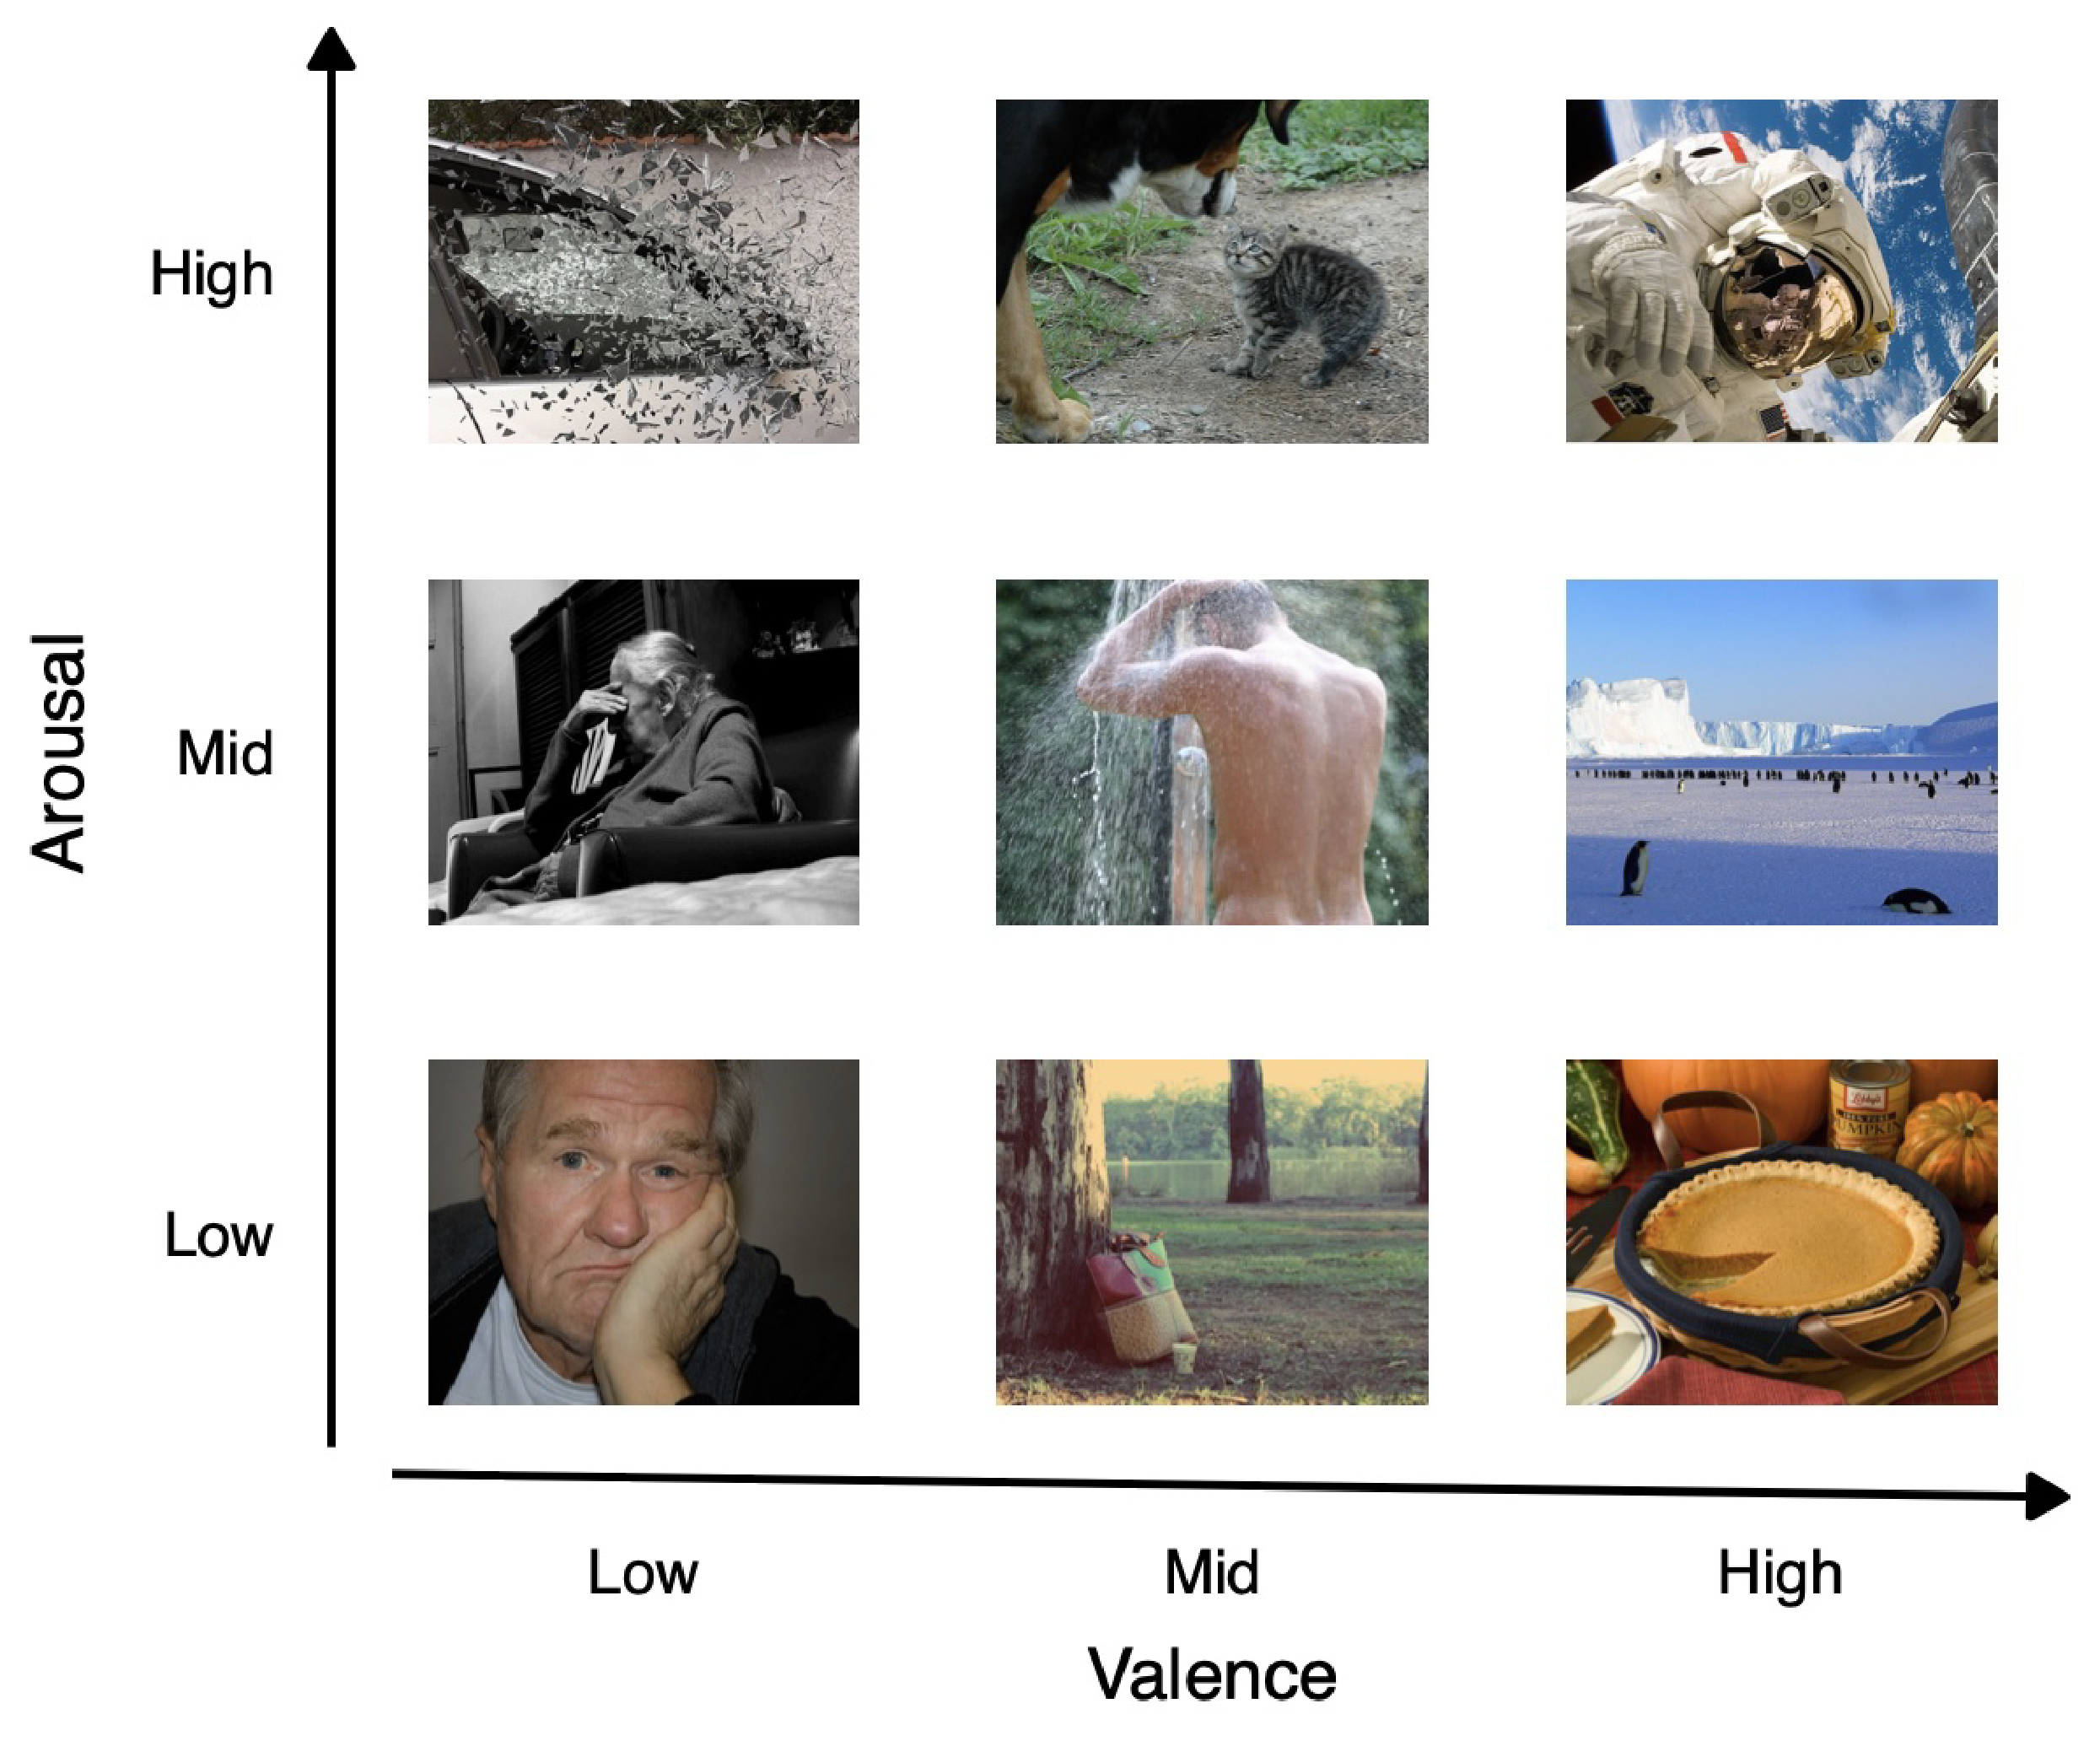
\includegraphics[width=0.82\textwidth]{plots/S1_OASIS_example.pdf}
  \caption{Representative images across the valence--arousal space for OASIS. Columns correspond to low, medium, and high valence; rows correspond to low, medium, and high arousal.}
  \label{fig:affective_space_examples}
\end{figure}

\begin{figure}[h]
  \centering
  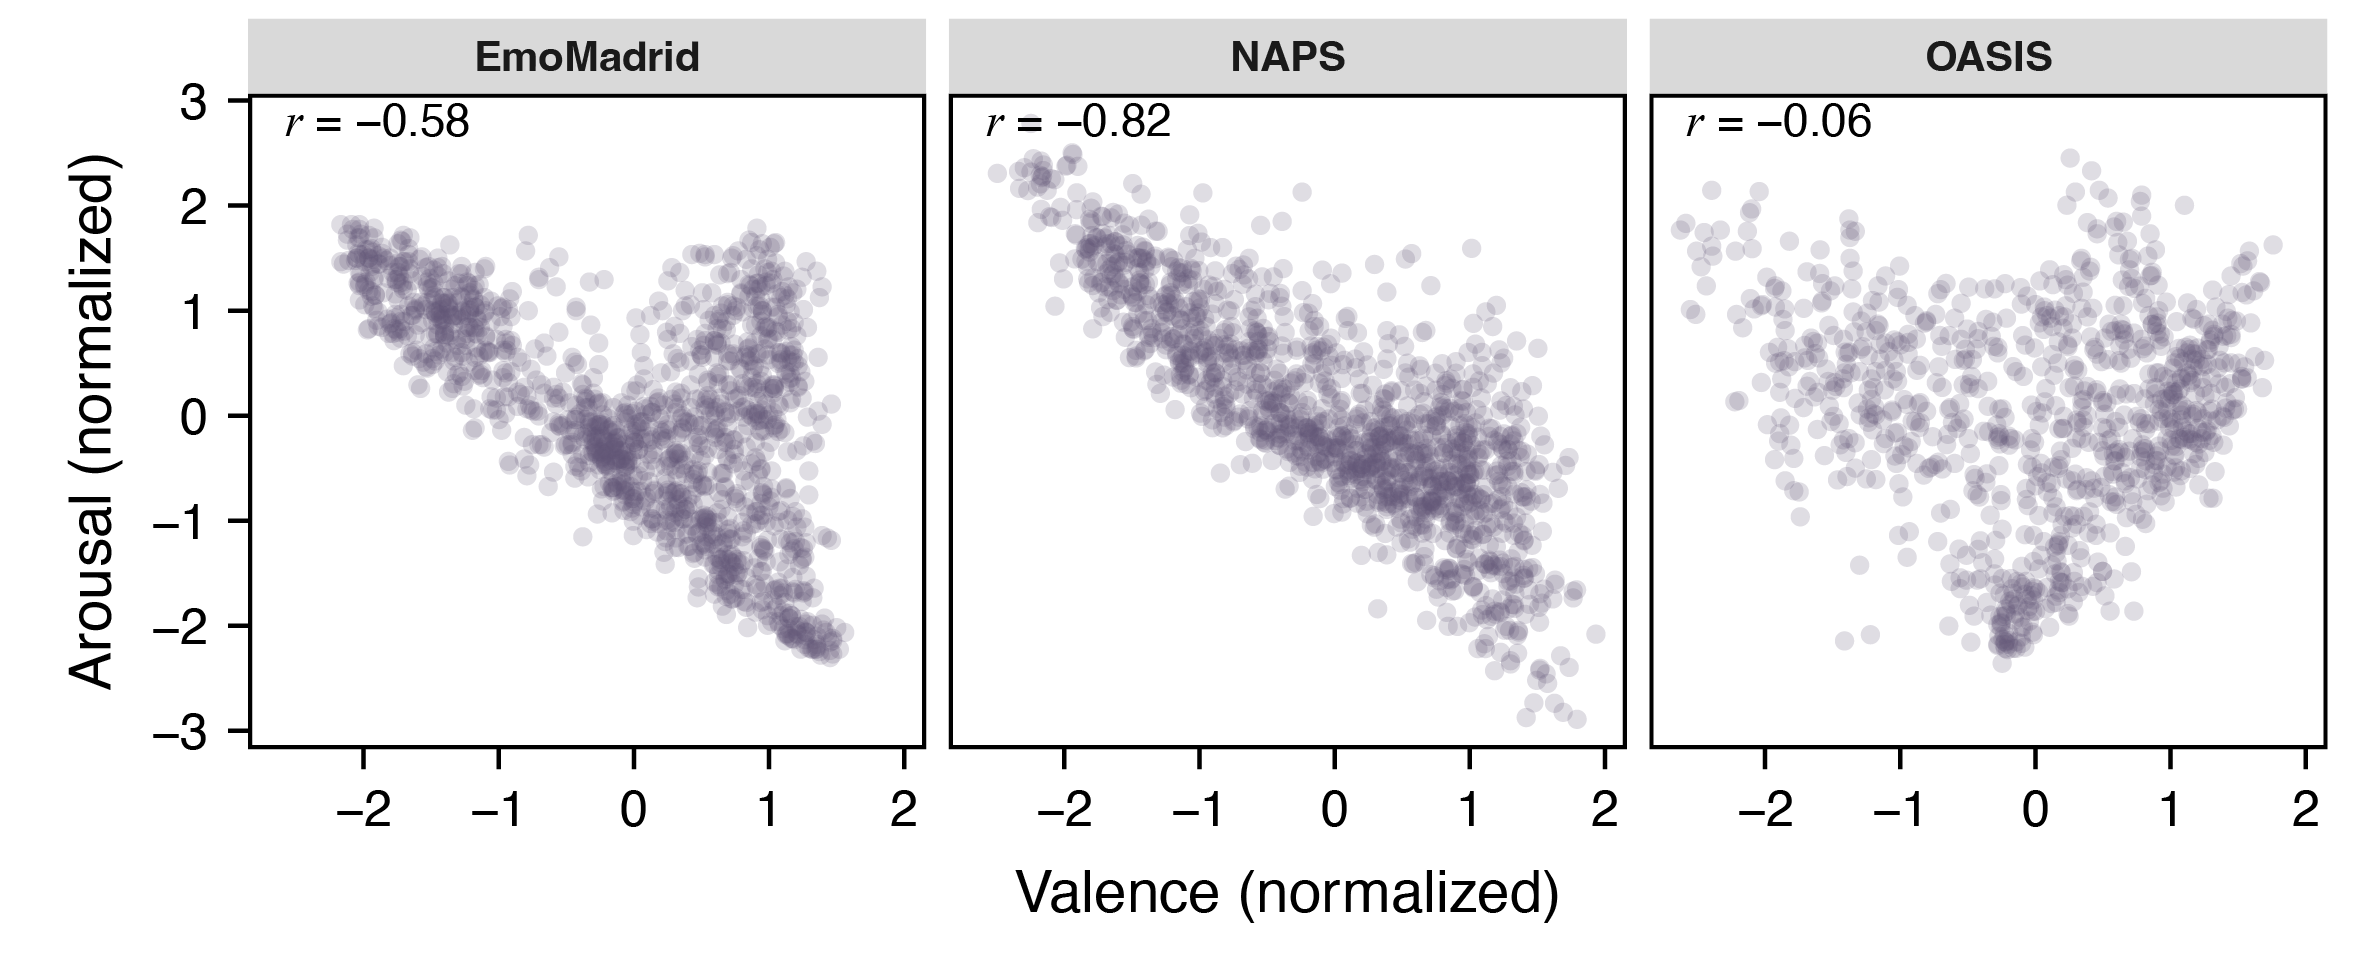
\includegraphics[width=\textwidth]{plots/S2_raw_landscape.png}
  \caption{Valence--arousal distribution for each dataset. Each point
    represents one image positioned by its normalized valence ($x$-axis)
    and arousal ($y$-axis). The Pearson correlation between valence and
    arousal is shown in each panel.}
  \label{fig:distribution}
\end{figure}

\begin{figure}[h]
  \centering
  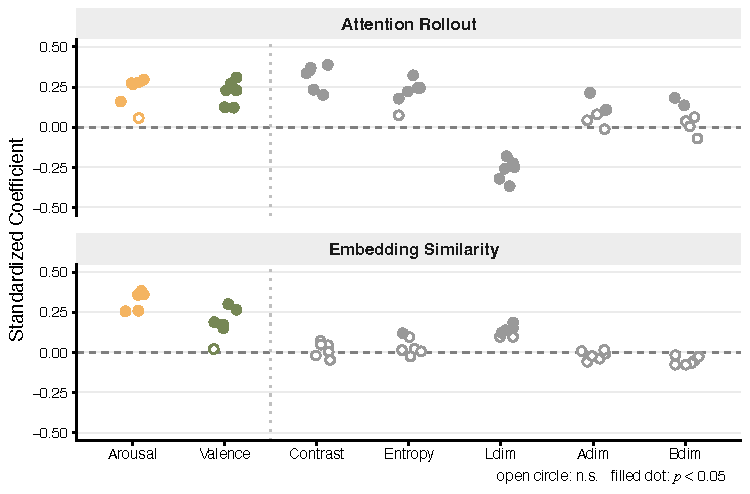
\includegraphics[width=\textwidth]{plots/S3-1_coef_EmoMadrid.pdf}
  \caption{Full regression coefficients for EmoMadrid, including all visual
    feature controls. Filled dots: Bonferroni-corrected $p < .05$;
    open circles: n.s.}
  \label{fig:coef_emomadrid}
\end{figure}

\begin{figure}[h]
  \centering
  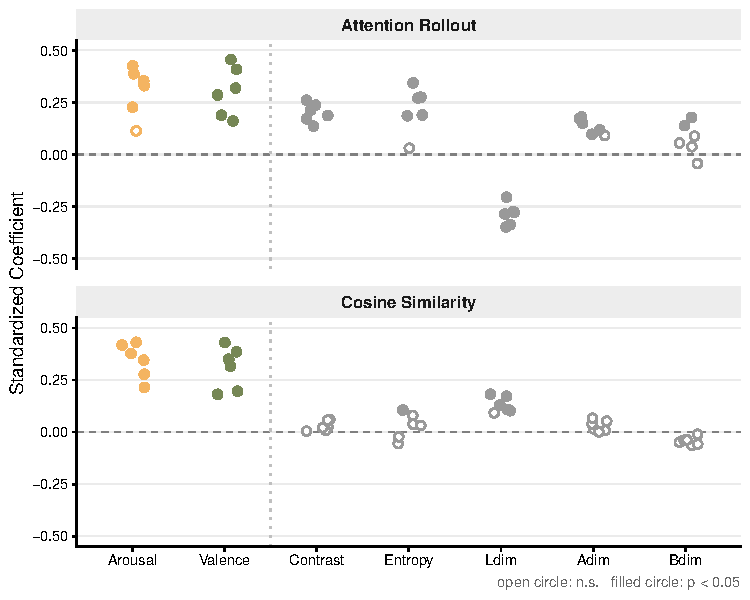
\includegraphics[width=\textwidth]{plots/S3-2_coef_NAPS.pdf}
  \caption{Full regression coefficients for NAPS, including all visual
    feature controls. Filled dots: Bonferroni-corrected $p < .05$;
    open circles: n.s.}
  \label{fig:coef_naps}
\end{figure}

\end{document}